\begin{surferPage}[216 Singularities]{משטחים בעלי מספר רב של נקודות סינגולריות ממשיות}
    כפי שכבר הזכרנו, המספר המרבי האפשרי
    $\mu(7)$ של נקודות סינגולריות במשטח ממעלה $7$ אינו ידוע.
    כל מה שיש לנו גבול עליון ותחתון: $99\le \mu(7) \le 104$. 


    על כן, אין זה מפליא שעוד פחות ידוע לנו על משטח כללי ממעלה $d$. 

    סוניה ברסקה, אוליבר לאבס ודוקו ון-סטראטן
    
    \textenglish{ (Breske, Labs, van-Straten)}הצליחו לשנות
    מבנה של ס.ו.\  צ'מוּטוֹב, כך שמספר נקודות הסינגולריות 
    המרבי שהתקבל נכון לעכשיו הושג גם כן באמצעות משטחים עם
    נקודות סינגולריות ממשיות. 
    נכון לעכשיו ידוע לנו ש:
    \[0,41\bar{6}d^3 \lessapprox \mu(d) \lessapprox 0.44\bar{4} d^3.\]
     במבט מלמעלה ניתן להבחין בסימטריה של המבנה ובקשר
    למספר המרבי של תאים שחורים בסידור של קווים:
    \begin{center}
      \begin{tabular}{c@{\qquad}c}
        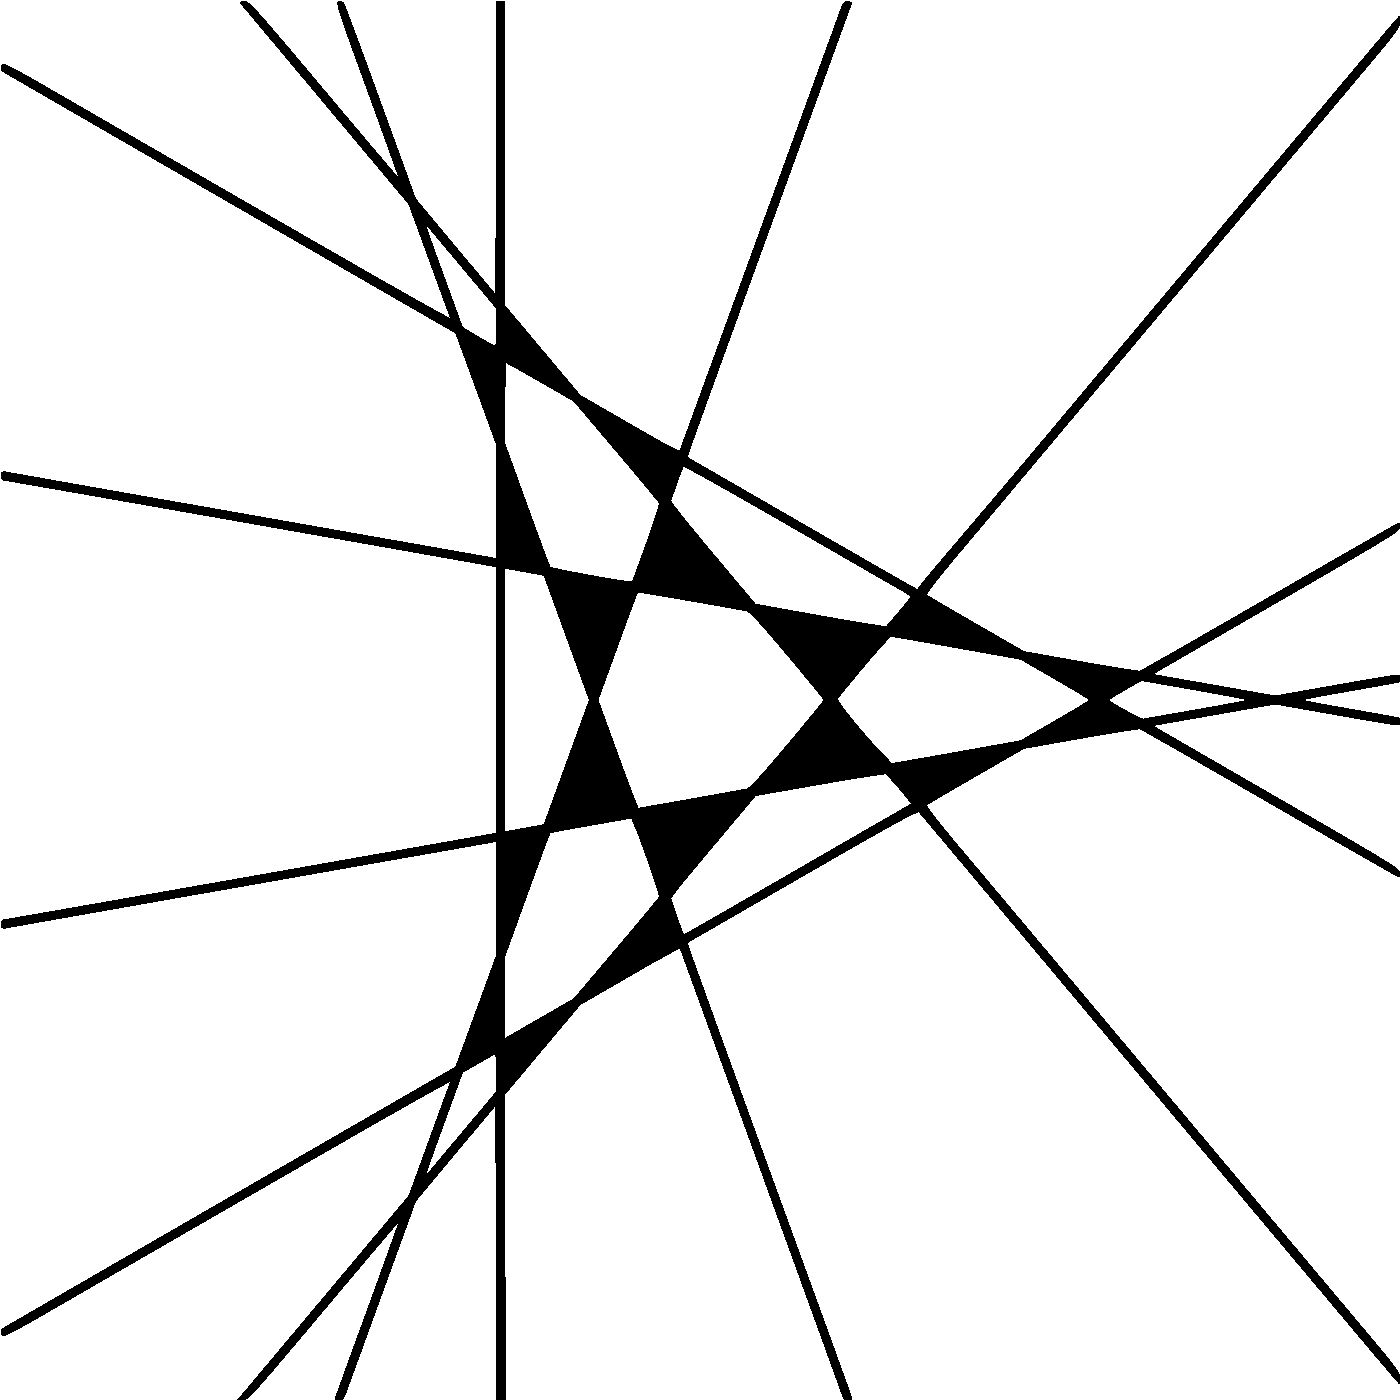
\includegraphics[height=1.5cm]{./../../common/images/vielesing.pdf}
        &
        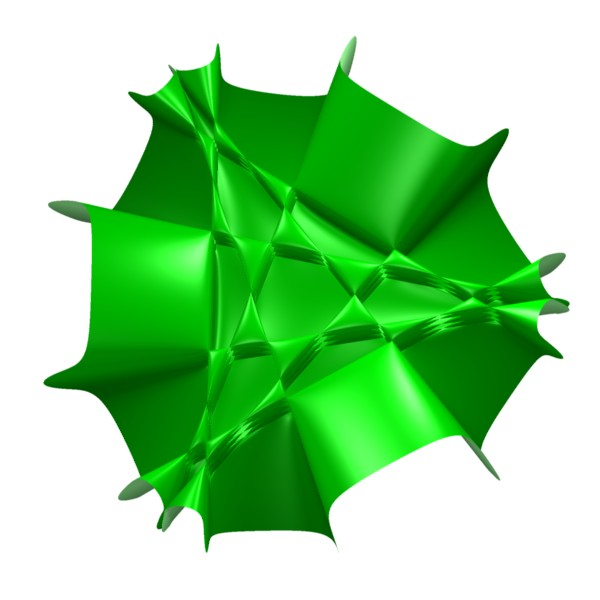
\includegraphics[height=1.5cm]{./../../common/images/p9surface_von_oben}
      \end{tabular}
    \end{center}
\end{surferPage}
